%%% mode: latex
%%% TeX-master: t
%%% End:

\chapter{绪论}
\label{cha:intro}


\section{研究背景与意义}
\label{sec:Background and meaning}
随着互联网技术的快速发展,特别是近十年来移动互联网的发展,设备之间的信息交流需求日趋旺盛。然而,在网络通信流量中,少数恶意流量掺杂在大量的正常流量中。这些恶意流量往往意味着未经授权的访问,若不加阻止就会导致信息泄露或破坏。因此,非常有必要部署一个高效准确的网络入侵检测系统,该系统能及时侦测到异常流量并采取相应措施。

入侵检测系统中检测部分是核心,网络中正常数据流量远大于恶意数据流量,检测的目标是减少对正常数据流量的误判以及提高对恶意数据流量的识别准确率。前者有助于减少网络中因误判导致的丢包,提高网络通信效率;后者可减少因恶意流量造成的损失,提供安全可靠的网络环境。

从广义上讲,网络入侵检测方法可分为两大类,第一类是基于签名的检测方法,即根据已知攻击类型生成流量特征数据库,根据当前检测到的流量特征在数据库中进行特征匹配,以判断网络流量的性质。第二类方法是基于异常的检测方法,此类方法克服了前一类只能检测已知类型攻击的局限性,可以检测零日攻击\cite{XXAQ202402001}。此类方法通常使用机器学习技术构建模型以判断流量的类别。

在基于机器学习的应用中,任务、数据集和方法三个要素不可或缺。任务是模型需要解决的具体问题,在入侵检测领域中通常是有监督学习的分类任务;数据集为模型提供了训练与测试所用的数据,高质量的数据集有助于提升模型性能;方法一般指模型的具体结构与调整模型中参数所使用的算法。

在实际部署中,最大的困难来自数据集。主要原因是在现实情况中,标注大量数据需要大量人力成本,而已开源数据集中的数据分布与实际情况相比存在一定的偏差。直接使用开源数据集训练所得到的模型,在实际部署中分类的准确性会有一定程度的下降。

为了解决这一问题,需要进行迁移学习。即首先在开源数据集上进行预训练,然后在实际数据集上进行微调。网络入侵检测数据集的形式可分为两种,原始的二进制流量或通过特定算法提取得到的统计特征。不同数据集的提取算法不同,因此得到的统计特征格式也各不相同,给迁移学习带来了困难。为了适应不同格式的数据集,部署者在进行迁移学习时需更改网络结构并重置对应的参数,在此过程中会造成已学知识的损失。且不同数据集都会提供描述该数据集格式的文档,该文档通常用于人工特征提取,已有的分类检测模型或迁移学习方法并没有充分利用文档中的信息。

针对上述的困难与不足,一种解决方法是利用多模态模型将数据及文档中的相关知识融入模型分类过程中。同时构建灵活、可兼容不同格式数据集的通用模型,以防止迁移学习过程中信息的损失。该多模态通用模型可以简化实际部署步骤,充分利用已有数据集中的信息,提高实际环境下模型分类的准确率。
\section{国内外研究现状}
\label{sec: Current research state}

网络入侵检测方法可分为两种,分别是基于签名的与基于异常的,后者常使用机器学习方法进行检测。入侵检测方法分类如图\ref{fig:research_review}所示。

\begin{figure}[htb]
\centering % 居中对齐子图
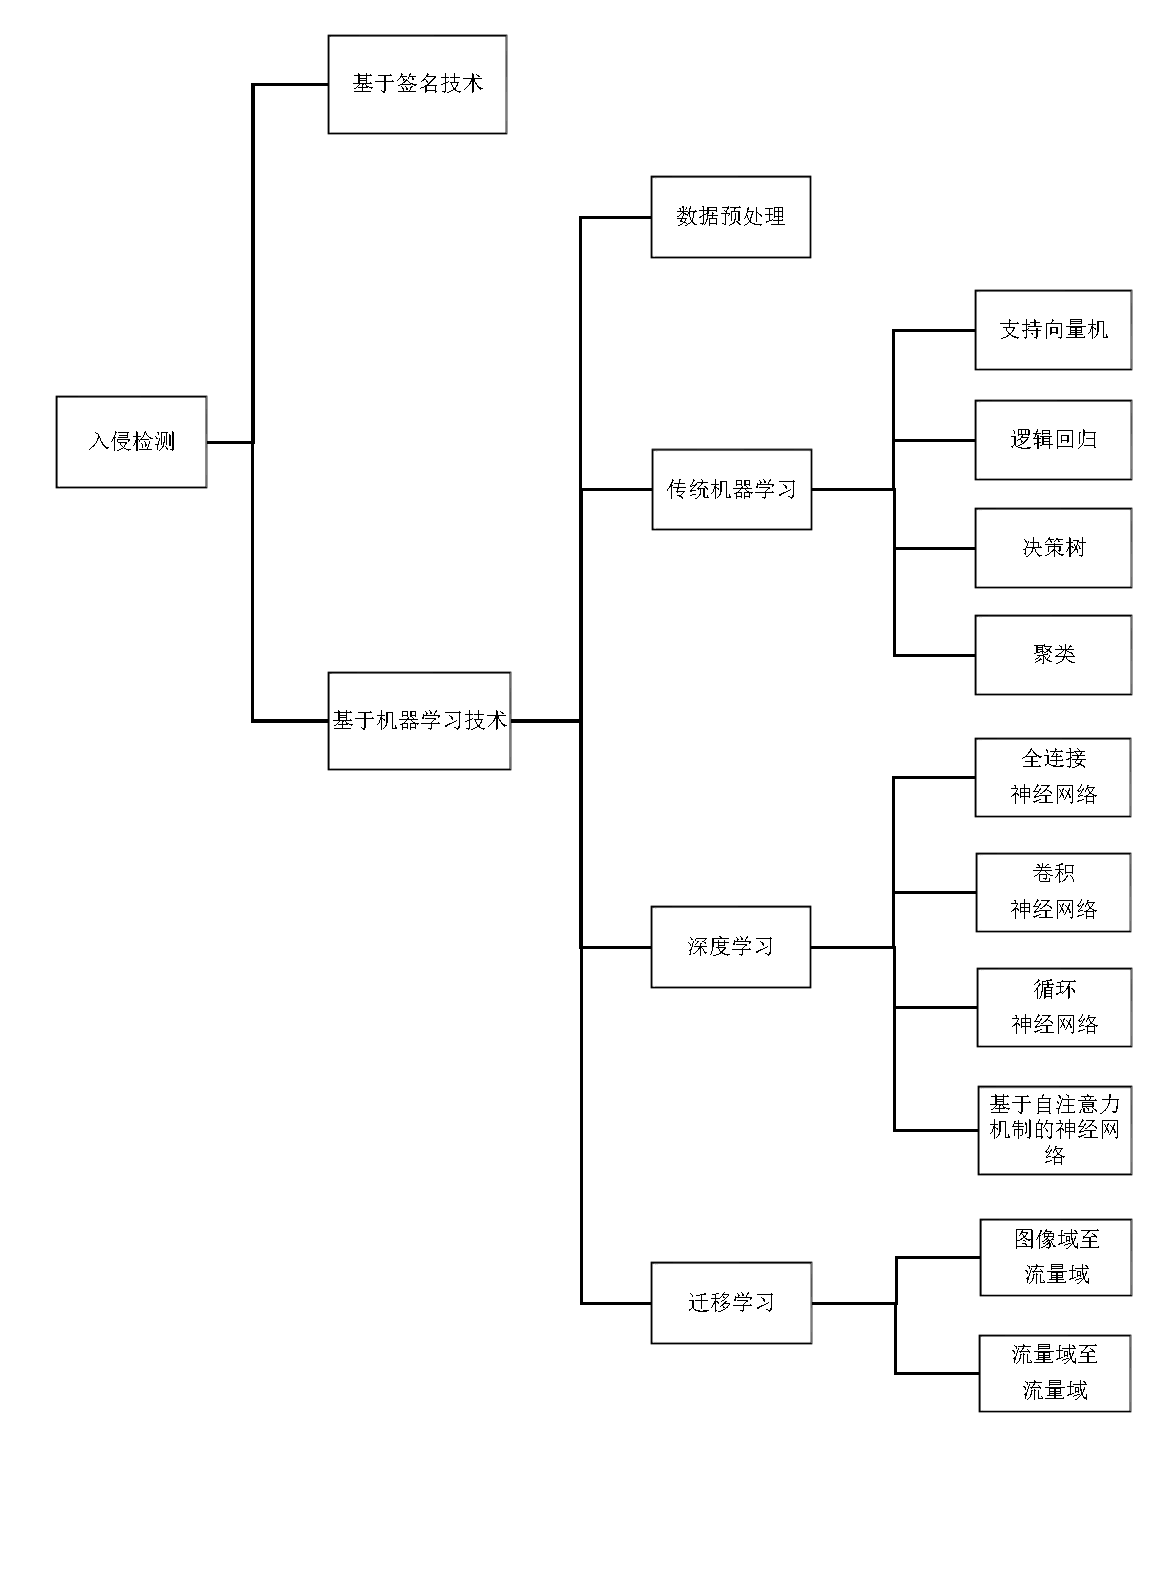
\includegraphics[width=.8\linewidth]{img/review.pdf} % 插入SVG图片
\caption{网络入侵检测方法分类}
\label{fig:research_review} % 子图的标签,用于交叉引用
\end{figure}%


\subsection{基于签名的网络入侵检测}
在基于签名的网络入侵检测系统中最重要的是签名数据库,该数据库由人工或机器根据已知的攻击模式提取特征并进行存储。入侵检测系统会对传入网络中的每一个数据包进行签名比对,一旦发现数据包特征与签名数据库中的特征匹配,入侵检测系统就会采取相应的防御措施。该方法广泛应用于商业防火墙软件中。在实际应用时,其灵敏度可根据实际情况进行调整,当设置为最高灵敏度时,虽然准确率最高,但会产生大量的误判。通过算法选择合适的签名,选出的签名可以保证在满足准确度要求的同时减少误报\cite{10.3390/app12020852}。基于签名的入侵检测技术可与基于机器学习的入侵检测相结合。使用蜜罐捕获网络攻击,随后使用机器学习分析捕获的流量,识别潜在恶意流量,对恶意流量实时生成签名并存储到数据库中,不断提高入侵检测系统的防御能力\cite{10.1007/s00521-019-04187-9}。
\subsection{机器学习数据预处理方法}
机器学习模型的性能上限由模型所学习数据的质量决定。为了保证模型能有效地从数据中学习,原始数据需要进行一系列预处理,从而转化为干净、格式统一的数据以便模型学习。原始数据分为结构化数据和非结构化数据。前者以表格形式呈现,有定义清晰的字段;后者没有固定格式,图像文字等属于此类。

在网络入侵检测任务中,结构化数据对应于通过指定算法抽取出的流量统计特征,而非结构化数据对应于原始的二进制网络流量数据。为提升机器学习中模型的学习效果以下是常用的数据预处理方法:
\begin{enumerate}
    \item 数值标准化。网络入侵检测中常用一种方法是最大最小值标准化方法,即将数值均匀地映射到[0,1]区间\cite{XAQY202212003,JSGG202206032,10.1016/j.csi.2023.103808,10.1080/21642583.2024.2321381,10.1109/ACCESS.2023.3251354}。另一种常见的方法是将样本各个属性转化为方差为1,均值为0的正态分布\cite{10.1016/j.ins.2021.03.060,10.1016/j.jksuci.2022.10.019}。对于分布范围很大的数据,取对数也是一种有效的标准化方法,可对数据范围进行显著压缩\cite{10.7717/peerj-cs.721}。
    
    \item 文字类型数据处理。网络流量特征中除了数值类型外,还包含文字类型数据,为方便处理此类数据,常使用的独热编码将其转换为稀疏二进制向量\cite{XAQY202212003,JSGG202206032,10.1016/j.csi.2023.103808,10.1016/j.measen.2022.100612,10.1016/j.knosys.2021.106798}。另一种方法是将文字类型转化为整数\cite{10.1016/j.simpat.2019.102031,10.1109/ICCSP48568.2020.9182099}。

    \item 对于网络数据包的负载部分,由于长度不同,可使用n-gram进行特征提取,该方法可将变长数据转化为定长向量\cite{10.1016/j.cose.2023.103171}。
    
    \item 网络流量的特征维度很高,对数据进行降维有助于提升模型表现,减少模型在学习过程中的过拟合现象。SelectKBest是一种常用特征选择方法,集成于scikit-learn库中,通过定义好的评分函数计算各个特征的重要性,以此选择最重要的k个特征实现降维\cite{10.1080/21642583.2024.2321381}。此外也可定义分数的阈值以选择最重要的特征\cite{10.1016/j.cose.2020.102062}。主成分分析是另一种根据阈值进行特征选择的方法,其选择方差最大的特征进行保留,从而将高维度数据投影至低维度\cite{10.1016/j.jksuci.2022.10.019}。计算数据各个分量之间的相关矩阵并剔除与目标变量(数据的类别)不相关或者彼此强相关的分量可以有效降维\cite{10.3390/math10030530}。自动编码器,也可以进行数据降维\cite{10.1016/j.knosys.2021.106798}。启发式算法也可进行特征选择,好的特征选择可以得到好的分类结果,于是可以将k近邻算法聚类效果作为评估函数,以选择最优特征子集\cite{10.1016/j.future.2020.07.042}。决策树算法如XGBoost 在进行分类时,实际上也实现了特征选择\cite{10.1016/j.comcom.2022.12.010,10.1016/j.icte.2020.03.002}。

    \item 网络流量数据存在显著的类别分布不均衡问题,即通常正常类别的样本数远大于异常类别样本数。直接在不平衡数据集上训练模型会缺少对小样本流量类别的识别能力,为重新平衡数据集可使用SMOTE(Synthetic Minority Over-sampling Technique)方法,通过对邻居样本采样合成新数据实现过采样\cite{PMID:34138657,10.7717/peerj-cs.721}。也可使用聚类增强过采样的效果\cite{XAXB202306010}。
    
\end{enumerate}
\subsection{基于传统机器学习的网络入侵检测}
\subsubsection{基于支持向量机的入侵检测}
支持向量机(Support Vector Machine, SVM)是一种监督学习方法。其核心思想是寻找最优超平面,该超平面能最大化不同类别数据之间的距离,理想情况下,不同类别之间的数据可以由一个超平面完美分隔开,但实际应用中数据分布较为复杂,并不是线性可分的。SVM通过使用核函数将样本映射到更高维度的空间,以获得更好的数据分布。样本个数是$n$的SVM在训练阶段的时间复杂度为$O(n^3)$,在处理网络入侵数据时可能成为性能瓶颈,可使用孪生支持向量机加快优化速度\cite{10.1109/ACCESS.2023.3251354}。

支持向量机在20年前就已经被应用到了入侵检测系统中\cite{10.1007/978-3-540-45235-5_73}。近年来使用支持向量机的入侵检测,都是将其与其他技术相结合提高支持向量机的性能,如使用高斯混合模型进行修正\cite{10.3390/electronics12040930},支持向量机可以用来替换深度学习中的softmax实现更好的分类效果\cite{PMID:37960661}。
\subsubsection{基于逻辑回归的入侵检测}
逻辑回归是机器学习中最简单最常用的模型,可根据输入变量判断其所属类别的概率。解决二分类问题时使用sigmoid函数,多分类问题则使用softmax函数。逻辑回归的最优参数常通过使用最大似然估计 得到。

入侵检测任务中可以使用其他启发式算法优化参数,如采用人工蜂群算法对逻辑回归的参数进行优化\cite{10.1016/j.csi.2023.103808}。偏最小二乘回归也可与逻辑回归进行结合,其具体分类流程是先对自变量进行降维,然后再用逻辑回归进行分类预测\cite{10.1007/978-981-33-4922-3_10}。
\subsubsection{基于决策树的入侵检测}
决策树由有向边和节点组成,节点分为两类,内部节点代表一种属性,叶节点代表具体类别。使用决策树对数据进行分类时,从根节点开始,数据都会根据每个内部节点对应的属性进行逐步划分,直至到达叶节点,即被划分为具体某一类别。对决策树进行模型集成,就可得到梯度提升决策树、随机森林等模型。

基于决策树的方法与其他机器学习方法进行结合,可克服单一模型的局限性。支持向量机很难用于解决多分类问题,将支持向量机嵌入到决策树内部结点中就可以解决入侵检测中的多分类问题\cite{10.1109/ACCESS.2023.3251354}。在数据集UNSW-NB15\cite{10.1109/MilCIS.2015.7348942}上进行数据降维后基于AdaBoost的决策树模型比简单的多层感知机或支持向量机效果要好\cite{10.3390/math10030530}。同时,在KDDCUP-99数据集上的研究,也表明决策树的性能优于逻辑回归和支持向量机\cite{10.1155/2021/6634811}。与支持向量机类似,决策树也可用于替代神经网络的softmax层以实现分类\cite{PMID:38339756}。对于多分类问题,也可以由不同的决策数分阶段进行决策,可以由两个决策树分别判断是否为恶意流量以及恶意流量对应的具体类别,然后由第3个决策树综合前两个决策树的分类结果输出最终分类结果\cite{10.3390/fi12030044}。

在进行集成学习的决策树模型上,可以使用其他方法进行二次集成,其中使用装袋法对集成了50个梯度提升机进行二次集成效果最好\cite{10.1016/j.eswa.2022.119030}。
\subsubsection{基于聚类的入侵检测}
聚类属于无监督学习即不需要样本的类别标签只需要样本特征,最基础的聚类算法是k均值聚类,其思想是通过迭代寻找若干中心点,每个中心点对应一种类别,最终使样本到所属中心点的距离最小。另一种实现聚类的方法是密度峰值聚类,但对于入侵检测这一种不均衡的数据集需要对其中密度峰值点的选择方法进行改进,让模型更重视稀疏区域\cite{10.1016/j.sysarc.2021.102212}。

对网络流量进行分类时,无监督聚类方法往往与其他有监督方法组合使用。聚类方法可以用在模型前端,使用k均值聚类进行第一步预分类,然后在每个聚类结果上分别训练随机森林分类器,这本质上也是一种模型集成方法\cite{10.1016/j.measen.2022.100612}。聚类也可以用在模型中间部分,分别对降维后的正常类别数据和异常类别数据进行两次聚类,然后将样本本身与距其最近的正常聚类中心和异常聚类中心组成二维数据,再使用卷积神经网络进行分类\cite{10.1016/j.knosys.2021.106798}。流量数据的特征分布较为复杂,在低维空间是线性不可分的,与支持向量机类似,可使用核函数,将其映射至容易线性可分的高维空间,使用多个核函数,可以让这一过程更简单\cite{10.1007/s13042-020-01253-w}。聚类的初始中心选择也非常关键,计算半相同(部分特征相似)实例集可以得到更好的聚类中心\cite{10.1016/j.cose.2020.102062}。除了通过不断迭代优化训练中心,也可以通过计算隶属函数确定某一样本是否属于已知集群以实现无监督聚类\cite{10.1007/s10699-019-09589-5}。神经网络也可应用到聚类过程中,为每个聚类中心配置一个神经网络,由该神经网络计算样本是否属于该类别可实现聚类\cite{10.1109/INFOCOM42981.2021.9488690}。

\subsubsection{传统机器学习存在的问题}
传统机器学习存在一定的局限性,特别是网络入侵领域,以下是对传统机器学习缺点的总结。
\begin{enumerate}
    \item SVM。SVM的性能很大程度上取决于核函数的选择,当更换数据集或数据集增加了新特征时,对模型进行调整较为困难。且SVM被设计用于二分类问题,异常网络流量可能有多个类别,这就需要设计多个SVM解决多分类问题,需要较多的计算资源。
    \item 逻辑回归。逻辑回归是一种线性模型,网络入侵检测中存在非线性特征,逻辑回归很难捕获复杂的攻击模式,其性能较差。
    \item 决策树。传统决策树算法,每个节点的特征选择与节点分裂都是根据整个数据集得到的,网络入侵检测中需要实时更新模型,而设计在线学习的决策树算法较为困难。另外,与SVM类似,决策树的结构与数据集密切相关,添加特征或更换数据集决策树往往会失效。
    \item 聚类。聚类是无监督的,识别每个簇代表的行为,需要进行额外的分析。在网络入侵检测中,由于数据不均衡,攻击流量可能会被视为噪音而被忽略。许多数据集提供了标签,而聚类方法是无监督的,并没有充分利用这些信息,其生成的模型效果较有监督模型差。
\end{enumerate}

深度学习是机器学习的一种,部分解决了上述存在的问题。深度学习在网络入侵检测领域的进展如下。

\subsection{基于深度学习的网络入侵检测}
\subsubsection{基于全连接神经网络的入侵检测}
多层感知机(Multilayer Perceptron,MLP)是一种人工神经网络,由一个输入层,多个隐藏层,以及一个输出层组成,两个相邻层之间的神经元相互连接,连接具有权值,每个神经元将连入它的连接加权求值,再使用非线性函数进行激活,激活后的值送入下一层。MLP是一种基础的神经网络架构,可用于监督学习任务,通常使用反向传播算法训练参数。

使用具有4个隐藏层,每个隐藏层具有100个节点的深度神经网络在KDDCUP-99数据集上具有最高性能,优于传统机器学习\cite{10.1049/iet-ifs.2018.5258}。


\subsubsection{基于卷积神经网络的入侵检测}
卷积神经网络与前一节所述的多层感知机相似,是对生物感知视觉方式的模仿,层与层之间没有全连接,而是使用卷积实现局部连接以及权值共享。一些数据集上相似的属性往往会放在相邻的位置,这就为使用卷积神经网络进行建模提供了方便。

随着ImageNet\cite{10.1109/CVPR.2009.5206848}数据集的提出,计算机视觉领域的神经网络架构研究取得了很多新的进展,因此只要将流量数据转化为图像,就可将用于视觉的网络架构应用到流量检测中。其中一种方法是将统计特征离散化转为二进制比特,然后将每8个二进制比特压缩为256灰阶像素,以此组成8×8的灰度图像使用ResNet等网络进行分类,该方法在NSL-KDD\cite{10.1109/CISDA.2009.5356528}数据集并未取得最好效果,但其优点在于无需进行特征选择\cite{10.1007/978-3-319-70139-4_87}。在将流量转化为图像的过程中,也可以不进行离散化,而是选择生成像素更多的图像\cite{PMID:34138657}。

除了转化为图像,也可使用一维卷积神经网络对流量数据直接进行分类。在此过程中,网络参数的设置非常重要,一种可行的解决方案是使用启发式算法进行优化,如粒子群算法对网络的结构进行搜索\cite{10.1016/j.ins.2021.03.060}。其他启发式算法如遗传算法也能进行网络搜索,搜索出的最优网络结构包含跨层连接\cite{10.1016/j.future.2020.07.042}。若不进行模型搜索,一种近似方法是使用多种尺寸的卷积以实现模型对流量的多尺度建模\cite{10.1016/j.future.2021.10.018}。

卷积网络除了对单个样本进行建模外,也可以进行局部时序建模\cite{10.7717/peerj-cs.721}。
\subsubsection{基于循环神经网络的入侵检测}
循环神经网络是用来进行时序建模的主流模型,传统的前馈神经网络如多层感知机和卷积神经网络,这些模型的输入尺寸都是固定的,无法处理变长的序列,而循环神经网络则将时序信息串行化,依次处理每一时刻的信息,且在处理时维护一个内部状态以记录之前的输入信息,实现对时序数据的感知。

最简单的结构是只使用循环神经网络,然后接全连接层\cite{10.1109/ICCSP48568.2020.9182099}。除了使用全部数据集中给出的特征,也可进行特征选择,只使用精简特征进行分类\cite{10.1016/j.comcom.2022.12.010,10.1016/j.icte.2020.03.002}。进行特征选择后,模型效果会好于使用全部特征且计算量更少内存占用更低\cite{10.1016/j.comnet.2023.109662}。使用去噪自编码器也可为循环神经网络提供降维后的特征\cite{XAXB202302002}。考虑网络流量类别的极度不均衡,可以由两个级联的递归神经网络进行分类,其中第一个检测是否为常见攻击类型,第二个检测是否为少见攻击类型\cite{10.1016/j.simpat.2019.102031}。

循环神经网络(Recurrent Neural Network,RNN)也可以与卷积神经网络搭配使用。常见方法是先使用若干层卷积神经网络提取网络流量的局部特征,然后再使用循环神经网络,提取网络流量的全局时序特征。不超过三层时,循环神经网络的层数越多效果越好,且使用长短期记忆网络(Long Short-Term Memory,LSTM)的效果最好,其次是门控神经单元(Gated Recurrent Unit,GRU),最差的是标准的RNN\cite{10.1109/ICACCI.2017.8126009,10.1016/j.comcom.2022.12.010}。为了充分利用这三种类型网络的差异性,可以使用并行结构将流量特征使用三种网络分别建模,然后进行降维,降维后再进行特征融合\cite{10.1016/j.compeleceng.2022.108156}。除了这三种基本结构,单循环单元(Simple Recurrent Unit,SRU)也可用于入侵检测,该神经单元的特点是采用了跳接思想以避免梯度消失,工业数据集上该方法确实优于GRU和LSTM\cite{10.1016/j.compeleceng.2021.107049}。在KDDCUP-99数据集上先使用三层卷积神经网络进行数据包的特征提取,然后再使用循环神经网络进行建模时发现:循环神经网络中长短期记忆网分类效果好,门控神经单元速度快,可以使用混合结构,在网络中的不同层次依次使用这两种网络,以实现更好的性能,考虑到循环神经网络的单向性,也可以由两层不同方向的网络对接起来,以实现双向时序建模\cite{10.1016/j.jksuci.2022.10.019}。对于这种具有复合结构的网络而言,超参数设置仍然很重要,因此可以通过使用遗传算法,对网络的超参数进行搜索\cite{10.1007/s11042-021-11271-7}。
最后得到分类结果,除了使用softmax或sigmoid函数计算外也可使用随机森林或支持向量机得出\cite{10.1016/j.compeleceng.2022.108156}。使用基于RNN的网络,可以构建自动编码器,根据重建结果与实际结果的差异值可判断是否为异常流量及恶意流量\cite{10.1109/TCAD.2020.3012749}。
\subsubsection{基于自注意力机制的入侵检测}
基于自注意力机制的神经网络模型中,最经典的是Transformer\cite{NIPS2017_3f5ee243},该模型主要由两部分组成,分别是多头自注意力机制以及其后的多层感知机,自注意力机制为该模型提供了全局建模能力以及对输入的灵活适应性。Transformer由两部分组成,分别是编码器和解码器。

最简单的方法是直接使用Transformer的原方案,对解码器的输出使用softmax函数得到样本对应的类别,该方案在相同推理时间的情况下,优于RNN和SVM\cite{10.1109/ACCESS.2022.3182333}。在仅使用编码器的情况下,其效果也优于RNN\cite{10.1016/j.comnet.2023.110072}。提取统计特征之后的流量数据,本质上是表格数据,因此可以使用TabNet进行分类\cite{PMID:37844095}。FlowTransformer框架对该Transformer应用到入侵检测中进行了探索,发现入侵检测任务比较简单,小模型与大模型的区别较小,影响模型性能的关键在于分类器的选择\cite{10.1016/j.eswa.2023.122564}。对卷积神经网络而言可将流量转化为图像,然后使用图像分类网络判断流量,对Transformer也是如此,但分类效果不如原生网络\cite{10.1109/ACCESS.2022.3200034}。网络流量有两种特征,分别是原始字节流和统计特征,可将这两种特征进行融合,对流量数据统一进行特征提取与分类\cite{10.1145/3511808.3557549}。使用多层感知机对传入Transformer的流量特征提前进行初步编码,可改善模型表现\cite{10.1016/j.cose.2023.103171}。对Transformer进行改进可以将其与卷积神经网络结合,先使用简单的卷积神经网络进行初步训练,将训练后的卷积层与Transformer相连,实现细粒度建模,在不同数据集上均优于传统模型\cite{10.1007/s11042-022-14121-2}。除了传统卷积,也可使用时序卷积以实现对局部时序信息的初步建模,该方法可以提升Transformer的性能\cite{10.1109/ACCESS.2022.3175516}。该方法也可与传统机器学习方法相结合,先使用决策树判断流量是否为恶意流量,然后再使用Transformer判断恶意流量具体的类别,级联后的方案比单独使用其中一种效果更好\cite{10.1109/ICDMW58026.2022.00081}。

\subsubsection{深度学习存在的问题}
上述四种深度学习方法存在一定的局限性,以下是对深度学习缺点的总结。
\begin{enumerate}
    \item 网络流量数据是时序数据,MLP缺乏时序建模能力。
    \item 将流量数据统计特征转化为图像会丢失信息。由于其感受野的局部性,单个网络流量中相距较远的两个特征的组合,需要通过多层卷积才能实现特征提取。
    \item 循环神经网络处理在处理长序列时存在梯度消失或梯度爆炸问题。
    \item 数据集中给出了每个特征对应的描述,模型并未充分利用。
\end{enumerate}

\subsection{迁移学习}
迁移学习,可以大体分为四类。第1类以TrAdaBoost\cite{10.1145/1273496.1273521}为代表,从源数据集中找到对目标任务有帮助的样本,从而实现前移学习。第2类方法以\cite{10.1109/TNN.2010.2091281}为代表,尝试将原数据集和目标数据集映射到同一个特征空间中,在映射过程中尽量减少数据信息的损失的同时,尽量让映射后的分布相同。第3类是在神经网络上进行迁移学习,其核心思想是重新利用已经在原数据集上训练好的参数,对源数据集上训练好的网络稍作修改即可用作目标数据集,如预训练的BERT\cite{10.18653/v1/N19-1423}。第4类是使用对抗性技术\cite{NIPS2006_b1b0432c}。当辨别器无法区分特征是来源于目标数据集还是原数据集,这说明了编码器提取的特征是同分布的。
\subsubsection{基于图像转换的网络流量迁移学习}
ImageNet是一个图像分类任务的数据集,它作为一个统一的标准,推进了人们对更有效网络结构的探索。在此任务上人们有丰富的方法与模型,如果能将网络流量数据转为图像,那就只需图像预训练模型即可完成迁移学习。TL-NID就是这么做的,它使用min-max标准化,然后将一维的序列折叠成二维的灰度图像再使用预训练的VGG-16实现迁移学习,效果比用决策树和随机森林好\cite{10.23919/ICITST51030.2020.9351317}。对于一些字符串类型的数据可以将其转化为独热编码\cite{10.1109/ACCESS.2020.2972627}。除了使用统计后的数据,也可以直接将二进制数据包按固定长度截断,把每个字节看成8-bit的灰度值,直接转化为图像,但预训练效果较差,可能是由于生成的图像与真实图像存在显著不同\cite{10.3390/info13120553}。直接使用灰度图像不利于特征的提取,在之前的基础上有人使用卷积将一维特征序列映射为RGB图像,然后使用模型集成的方法对流量进行判断\cite{10.1109/ACCESS.2022.3233775}。流量特征也可以通过三种降维方式(PCA、t-SNE和KPCA)生成三个通道对应彩色图像的RGB\cite{10.1016/j.future.2021.07.015}。TDL-IDS\cite{10.1109/GLOBECOM48099.2022.10001267}则是充分考虑了数据包之间的时序关系,采用LSTM进行建模,在NSL-KDD上训练后,冻住部分隐藏层然后在AWID数据集上微调。另一种迁移学习的方法则是先使用卷积神经网络学习粗略的特征,然后在第二阶段冻住网络,在后面添加新的网络实现对目标数据集上特征的准确提取\cite{10.1109/ICBDA.2019.8713213}。

\subsubsection{基于网络流量特征的迁移学习}
除了把数据转化为图片,然后使用图像分类,对网络进行流量分类也可以直接对流量进行处理。使用普通的全连接层搭建神经网络进行迁移学习,具体方法是先在原数据集上进行训练,然后重置Softmax层再在目标数据集上进行微调,但该实验提出的方法只能处理同样结构的数据\cite{10.1109/SMARTCOMP.2019.00031}。另一个方法是优化两个矩阵,使源数据集和目标数据集都可以通过投影矩阵投影到一个相同的子空间\cite{10.1109/MILCOM.2017.8170749}。从原始的二进制网络流量出发,对不同数据集提取相同格式的特征,然后使用卷积神经网络,在其中一种上进行训练,随后冻结训练好网络中的上半部分再在定目标数据集上对训练好的网络进行微调,可以实现迁移学习 \cite{10.1016/j.eswa.2022.118641}。

\subsubsection{迁移学习存在的问题}
上述两种迁移学习存在一定的局限性,以下是对迁移学习缺点的总结。
\begin{enumerate}
    \item 将网络流量转化为图像时,生成的图像与自然图像不同,可能会导致模型难以准确提取数据的特征,限制模型性能。
    \item 将流量数据统计特征转化为图像,实际上进行了升维,需要更大的存储空间,转化过程也需要消耗大量计算资源。
    \item 直接进行迁移学习时,若数据集的格式发生变化,需要重置投影层或使用新的投影矩阵。这些抛弃的参数中含有模型里学到的信息,迁移过程中,这些信息并没有被迁移到新模型中。
\end{enumerate}

\subsubsection{研究挑战与科学问题}
根据国内外研究现状,入侵检测领域的研究挑战是:
\begin{enumerate}
    \item 网络流量数据中存在多种模态(数值、文本等)的数据,如何如何充分融合这些数据以及描述信息对提升模型检测能力较为重要,而当前缺少合适的融合方法。
    \item 公共数据集与现实存在区别,当在实际环境中部署公共数据集训练得到的模型,其检测性能会下降。基于模型的迁移学习中存在损失,这会降低迁移效果。减少信息损失对模型设计以及迁移方法提出了更高要求。
\end{enumerate}

针对上述挑战,本文要解决的科学问题是如何解决公共数据集与实际数据的差异导致模型性能下降的问题。

\section{本文主要研究内容}
\label{sec:Research content for this paper}
\subsection{研究目标}
针对本文在入侵检测领域要解决的科学问题,研究目标如下:
\begin{enumerate}
    \item 设计新的映射方法将端口值、协议类型等字段进行更合理的映射。该映射与数据集无关,与上述字段的含义有关,减少了迁移时模型参数的信息损失。
    \item 利用Transformer的多模态建模能力,将数据集中的文字描述部分融入模型的特征提取与分类过程中,实现语言信息辅助建模,提高分类准确率。将建模后的信息进行时序特征提取,进一步提高分类的准确率。
    \item 使用通用模型,在不同数据集之间进行迁移学习,在迁移过程中减少模型的修改,尽可能保留已学习的参数。同时相比传统迁移学习方法,使用通用模型的分类方法具有更高准确率。
\end{enumerate}

\subsection{具体工作}

从上述研究目标出发,本文构建的多模态通用入侵检测系统如下图示,其主要由三个部分构成,分别是数据预处理,模型训练与推理,结果批量导出。
\begin{enumerate}
    \item 数据预处理部分的工作主要有两部分,对于文字部分需要将文本转化为对应的向量,对于数值部分则需要通过一定的算法将其转化为较小的分布范围,帮助模型学习其中的特征。同时将数据集中描述部分转化为句子表征向量。
    \item 利用Transformer的多模态能力在位置编码部分引入语义信息。
    \item 构建通用编码器同时引入以及进行时序建模,在建模过程中引入数据集中的表征向量,提高模型对不同数据集的适应性减少迁移学习时的信息损失。

\end{enumerate}

\section{论文组织结构}
\label{sec:Paper organization structure}
论文共有六个章节,组织结构如下:

第1章 绪论。简要说明了网络入侵检测领域所研究的内容,以及国内外对于机器学习在入侵检测中的最新研究进展,总结了当前研究方法存在的局限性,并进一步说明本文研究的内容以及提出的方法。

第2章 数据预处理与数据增强。介绍所用数据集并对数据集的特点进行分析,根据分析结果对数据集给出了相应的预处理方法以及数据增强方法。

第3章 基于多模态的入侵检测。提出了一种基于Transformer的通用入侵检测模型,说明了引入语言信息辅助建模的具体思路,介绍了实验平台设置以及入侵检测中常用的评价指标,在CIC-IDS2017数据集上进行了相关实验并对位置编码进行可视化分析。

第4章 基于时序建模的入侵检测。在多模态模型的基础上进行时序建模,将实验结果与近期入侵检测领域的研究进展进行了对比并对时序上的注意力进行了可视化分析。

第5章 基于迁移学习的入侵检测。给出了将时序多模态模型迁移至目标数据集上的实现方法,并使用两个数据集进行试验,比较了两种迁移学习方法。

第6章 总结与展望。总结了本文提出的多模态通用检测方法并分析了方法存在的不足,给出了未来可能改进的方向。
